\documentclass[12pt]{report}
\usepackage[utf8]{inputenc}
\usepackage[russian]{babel}
%\usepackage[14pt]{extsizes}
\usepackage{listings}
\usepackage{graphicx}
\usepackage{amsmath,amsfonts,amssymb,amsthm,mathtools} 
\usepackage{pgfplots}
\usepackage{filecontents}
\usepackage{indentfirst}
\usepackage{eucal}
\usepackage{amsmath}
\usepackage{enumitem}
\usepackage{fixltx2e}
\usepackage{float}

\frenchspacing

\usepackage{indentfirst} % Красная строка


%\usetikzlibrary{datavisualization}
%\usetikzlibrary{datavisualization.formats.functions}

\usepackage{amsmath}


% Для листинга кода:
\lstset{ %
language=caml,                 % выбор языка для подсветки (здесь это С)
basicstyle=\small\sffamily, % размер и начертание шрифта для подсветки кода
numbers=left,               % где поставить нумерацию строк (слева\справа)
numberstyle=\tiny,           % размер шрифта для номеров строк
stepnumber=1,                   % размер шага между двумя номерами строк
numbersep=5pt,                % как далеко отстоят номера строк от подсвечиваемого кода
showspaces=false,            % показывать или нет пробелы специальными отступами
showstringspaces=false,      % показывать или нет пробелы в строках
showtabs=false,             % показывать или нет табуляцию в строках
frame=single,              % рисовать рамку вокруг кода
tabsize=2,                 % размер табуляции по умолчанию равен 2 пробелам
captionpos=t,              % позиция заголовка вверху [t] или внизу [b] 
breaklines=true,           % автоматически переносить строки (да\нет)
breakatwhitespace=false, % переносить строки только если есть пробел
escapeinside={\#*}{*)}   % если нужно добавить комментарии в коде
}

\usepackage[left=2cm,right=2cm, top=2cm,bottom=2cm,bindingoffset=0cm]{geometry}


% plot
\usepackage{pgfplots}
\usepackage{filecontents}
\usetikzlibrary{datavisualization}
\usetikzlibrary{datavisualization.formats.functions}

\graphicspath{ {img/} }


\usepackage{subcaption}
\DeclareCaptionLabelSeparator{custom}{. }
	
\captionsetup
{
    labelsep=custom
}


\begin{document}
	\begin{titlepage}
		\thispagestyle{empty}
		
		\noindent
		\begin{minipage}{0.15\textwidth}
			
\includegraphics[width=\linewidth]{main_logo}
		\end{minipage}
		\noindent
		\begin{minipage}{0.9\textwidth}
			\centering
			\textbf{Министерство науки и высшего образования Российской Федерации}\\
			\textbf{Федеральное государственное бюджетное образовательное учреждение высшего образования}\\
			\textbf{«Московский государственный технический университет имени Н.Э.~Баумана}\\
			\textbf{(национальный исследовательский университет)»}\\
			\textbf{(МГТУ им. Н.Э.~Баумана)}
		\end{minipage}
		
		\noindent
		\rule{18cm}{3pt} %пустая строка
		\newline\newline %пустая строка
		\noindent ФАКУЛЬТЕТ $\underline{\text{«Информатика и системы управления»}}$ \newline\newline
		\noindent КАФЕДРА $\underline{\text{«Программное обеспечение ЭВМ и информационные технологии»}}$\newline\newline\newline\newline\newline
		
		
		\begin{center}
			\noindent\begin{minipage}{1.3\textwidth}\centering
				\Large\textbf{РАСЧЕТНО-ПОЯСНИТЕЛЬНАЯ ЗАПИСКА К}\newline
				\Large\textbf{НАУЧНО-ИССЛЕДОВАТЕЛЬСКОЙ РАБОТЕ}\newline
				\Large\textbf{НА ТЕМУ:}\newline
				\textbf{"Классификация известных методов}\newline
				\textbf{противодействия мошенничеству в}\newline
				\textbf{области больших данных"}\newline\newline
			\end{minipage}
		\end{center}
		
		\noindent\textbf{Студент} $\underline{\text{Коняев Е.А}}$\newline\newline
		\noindent\textbf{Группа} $\underline{\text{ИУ7-53Б}}$\newline\newline
		\noindent\textbf{Научный руководитель} $\underline{\text{Гаврилова Ю.М.}}$\newline\newline
		\noindent\textbf{Подпись руководителя}$\underline{\text{~~~~~~~~~~~~~~~~~~~~~~~~~~~}}$\newline\newline
		
		\begin{center}
			\vfill
			Москва~---~\the\year~г.
		\end{center}
	\end{titlepage}
	
	\setcounter{page}{2}
	\tableofcontents
	
	\newpage
	\chapter*{Введение}
	
	\addcontentsline{toc}{chapter}{Введение}
	
	
	Существуют различные типы рисков в финансовой сфере, такие как финансирование терроризма, отмывание денег, мошенничество с кредитными картами и мошенничество со страховкой, которые могут 
	привести к катастрофическим последствиям для таких организаций, как банки или страховые компании. Причем экономические последствия мошенничества могут быть более серьезными, чем просто
материальные затраты. Не менее значимыми показателями убытков от мошенничества являются потеря репутации, потеря доверия потребителей, потеря налогового дохода и т.д. Именно поэтому крайне важно противостоять мошенничеству в финансовой сфере.

	Вышеописанные финансовые риски обычно выявляются с помощью алгоритмов классификации. В задачах классификации асимметричное распределение классов, также известное как дисбаланс классов, является очень распространенной проблемой при обнаружении финансового мошенничества, когда для решения этой проблемы используются специальные подходы к анализу данных наряду с традиционными алгоритмами классификации. Эта проблема становится более значительной, когда мы рассматриваем область Big Data, методы которой применяются для анализа баз данных в финансовой сфере, так как обычноми методами обработки реляционных таблиц это уже невозможно сделать в силу масштабности пользовательских данных. Поэтому важно при выявлении мошеннических действий правильно вибрать методы анализа из области BigData, которые будут эффективны для данной задачи.
	
	С учетом всего вышесказанного, целью данной является анализ известных методов противодействию мошенничества в области BigData. Для этого необходимо:
	\begin{enumerate}
		\item[1)] провести анализ предметной области;
		\item[2)] сформулировать критерии оценки известных методов методов;
		\item[3)] провести обзор методов;
		\item[4)] классифицировать методы.
	\end{enumerate}

	\chapter{Аналитическая часть}
	
	\section{Анализ предметной области}
	
	\section{Общая характеритика Big Data}
	
	Термин «Big Data» означает большие работы (коллекции, потоки) данных, которые не могут быть обработаны традиционными компьютерными техниками. Этот термин означает не само понятие «большие данные», а предмет исследования, который включает в себя различные инструменты, техники и платформы.
	
	Большие данные включают в себя информацию, генерируемую различными системами и приложениями. Некоторые из сфер, которые попадают под определение «Big Data»:
	\begin{enumerate}
		\item[1)] черный ящик: информационная составляющая часть вертолета, самолета, морского/космического корабля. Данные подобного рода включают в себя запись голосов экипажа (микрофоны и наушники), информацию о характеристиках объекта управления;
		\item[2)] социальные медиа: включают данные, распространяемые через социальные сети;
		\item[3)] фондовые биржи: хранение информации о сделках купли-продажи между копаниями-партнерами;
		\item[4)] транспортные системы: модели, характеристики, расстояния  - все информация о транспорте и дорожных сетях.
		\item[5)] и т.п.
	\end{enumerate}
	
	Как следствие, термин «Big Data» включает большое объем, высокую скорость обработки и широкое разнообразие данных и делится на три типа:
	\begin{enumerate}
		\item[1)] структурные данные – реляционные БД;
		\item[2)] полу-структурированные данные – XML-файлы;
		\item[3)] неструктурированные данные – файлы формата Word, PDF, Text, медиа-журналы.
	\end{enumerate}

	Для использования возможностей больших данных требуется инфраструктура, которая может управлять и обрабатывать огромные объемы структурированных и неструктурированных данных в реальном времени. Существуют два класса техники, которые обрабатывают большие данные: технологии обработки Big Data и программно-аппаратные средства работы с большими данными.

	Технологии обработки Big Data:
	\begin{enumerate}
		\item[1)] модель распределенных вычислений MapReduce;
		\item[2)] технологии Hadoop;
		\item[3)] подход NoSQL;
		\item[4)] язык программирования R.
	\end{enumerate}
	
	Программно-апаратные средства работы с Big Data:
	\begin{enumerate}
		\item[1)] комплекс инструментов Oracle Exalytics;
		\item[2)] аппаратно-программный комплекс SAP HANA;
		\item[3)] IBM Watson Explorer.
	\end{enumerate}
	
	\section{Обнаружение мошенничества в области Big Data}
	
	Аналитика мошенничества на основе больших данных является эффективным подходом по трем причинам. Эти причины сводятся к следующему:
	\begin{enumerate}
		\item[1)] \textbf{точность}. Большинство организаций имеют ограниченные возможности для проверки случаев мошенничества человеком. Цель аналитики мошенничества на основе данных состоит в том, чтобы наиболее оптимально использовать имеющиеся ограниченные возможности или в другими словами, чтобы максимизировать долю мошеннических дел среди проверенных (и возможно обнаруженную сумму мошенничества);
		\item[2)] \textbf{операционная эффективность}. Аналитика мошенничества на основе данных построена с использованием методов из различных областей, включая машинное обучение, статистику, математику, глубокое обучение. Это значительно повышает эффективность работы что критически важно для многих сценариев мошенничества. Например, при оценке транзакция с кредитной картой, требуется почти немедленное решение относительно одобрить или заблокировать транзакцию из-за подозрения в мошенничестве;
		\item[3)] \textbf{экономичность}. Разработка и поддержка эффективной и экономичной системы обнаружения мошенничества, основанной на человеческих русурсах, является сложной и трудоемкой задачей. Более автоматизированный и более эффективный подход к разработке и обслуживанию системы обнаружения мошенничества является подход, основанный на анализе больших данных.
	\end{enumerate}
	
	Подводя итог вышесказанному, становится очевидно, что аналитика мошенничества на основе данных имеет много преимуществ по сравнению с традиционным экспертным подходом к обнаружению мошенничества. Однако в этом методе обнаружения мошенничества существуют различные проблемы, которые необходимо решить или минимизировать, чтобы усилить эффективность такой системы. Одной из таких критических проблем является проблема дисбаланса классов.
	
	\section{Проблема дисбаланса классов}
	
	Проблема дисбаланса классов — одна из самых серьезных проблем. Она определяется как чрезвычайно несбалансированное и сильно перекошенное распределение данных. Другими словами, соотношение мошеннических или преступных действий значительно меньше, чем законных и подлинных. Рисунок \ref{schema_imbalance_classes} иллюстрирует проблему дисбаланса классов, обнаруженную при выборке большого объема транзакционных операций в сфере кредитования, где коэффициент дисбаланса составляет 5,96\%. Красные точки на рисунке обозначают случаи мошенничества, частота которых намного ниже, чем у других случаев.
	
	\begin{figure}[H]
		\centering
		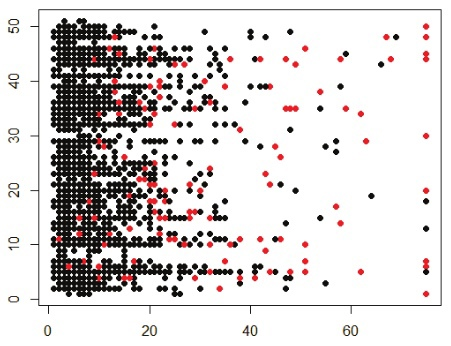
\includegraphics[width=0.8\linewidth]{imbalance_classes}
		\caption{Схема, иллюстрирующая проблему дисбаланса классов}
		\label{fig:schema_imbalance_classes}
	\end{figure}
	
	Несбалансированность классов усложняет определение характеристик мошеннических действий и выявление моделей мошенничества. Из-за доминирования одного класса большинство шагов оптимизации (относительно точности), выполняемых алгоритмом классификации, направлены на то, чтобы правильно классифицировать доминирующий класс, игнорируя другие. В этом случае наблюдения меньшинства являются наиболее важными для правильной классификации. Если алгоритм классификации не может обнаружить схемы мошенничества, незаконные операции считаются законными, что наносит серьезный финансовый ущерб.
	
	Многие исследования были посвящены этой проблеме. Было предложено несколько решений (например, [??]), которые построены на алгоритмах машинного обучения и интеллектуального анализа данных. Однако, подходы, обычно используемые для решения проблем дисбаланса, могут иметь неприятные последствия. Они улучшают чувствительность, но улучшение приводит к увеличению количества "ложных тревог". Таким образом, используя несбалансированные подходы к классификации, количество генерируемых ложных случаев выше, чем количество выявленных случаев мошенничества.
	
	\begin{Выбор критериев оценивания}
	Как правило, точность является наиболее распространенной мерой эффективности в задаче классификации. Однако в рассматриваемой задаче точность недостаточна из-за несбалансированной классификацией, и использование только ее в качестве меры эффективности приведет к искаженным результатам. Процент мошенничества довольно невысок от общего числа операций. Это означает, что степень точности классификации менее 95\% или 88\% соответственно неприемлема просто потому, что случайный классификатор способен достичь высокой точности в случае классификации с дисбалансом. Обнаружение мошенничества может оказаться недостижимым при достижении высокой степени точности. Поэтому мы рассмотрим другие показатели производительности, в частности чувствительность, площадь под кривой точности-отзыва (AUPC) и показатель F1. Мы предоставляем подробную информацию о нашем процессе выбора. Для оценки методов, представленных в данной диссертации, путаница в матрице вида, представленного в таблице 1.2, вычисляется с использованием тестовых наборов путем сравнения прогноза метода с фактическим значением. 

	
\addcontentsline{toc}{chapter}{Список использованных источников}

\nocite{*} 

\renewcommand\bibname{Список использованных источников} % переименовать страницу списка литературы
\bibliographystyle{utf8gost705u}  % стилевой файл для оформления по ГОСТу
\bibliography{lib}          % имя библиографической базы (bib-файла)
	
\end{document}
